\documentclass[a4paper]{report}

\usepackage[utf8]{inputenc}
\usepackage[english]{babel}
\usepackage[T1]{fontenc}
\usepackage{textcomp}
\usepackage[]{amsthm} 
\usepackage[]{amssymb}
\usepackage{amsmath}
\usepackage{graphicx}
\usepackage{float}
\usepackage{soul}
\usepackage{color}
\usepackage{bm}
\usepackage{listings}
\usepackage{xcolor}
\usepackage{enumitem}
%\usepackage{xfrac}
\usepackage[normalem]{ulem}

\usepackage[colorlinks=true, linkcolor=blue]{hyperref}

\usepackage{tikz}
\usetikzlibrary{trees}
\usetikzlibrary {fit,shapes.geometric} % W: Command terminated with space. (1)
\usetikzlibrary {automata} % W: Command terminated with space. (1)
\usetikzlibrary{arrows.meta}
\usepackage{multicol}

\usepackage{algorithm}
\usepackage[noend]{algpseudocode}
\usepackage{caption}

\usepackage{pgfplots}
\pgfplotsset{compat = newest}

\usepackage{geometry}
\geometry{legalpaper, margin=1in}

\renewcommand{\labelitemii}{$\circ$}
\renewcommand{\labelitemiii}{$\star$}
\renewcommand{\labelitemiv}{$>$}

% figure support
\usepackage{import}
\usepackage{xifthen}
\pdfminorversion=7
\usepackage{pdfpages}
\usepackage{transparent}
\newcommand{\incfig}[1]{%
    \def\svgwidth{\columnwidth}
    \import{./figures/}{#1.pdf_tex}}

% Newline for algorithm psuedo
\newcommand{\algrule}[1][.2pt]{\par\vskip.5\baselineskip\hrule height #1\par\vskip.5\baselineskip}

% -------- Listings/XColor Settings --------
\definecolor{codegreen}{rgb}{0,0.6,0}
\definecolor{codegray}{rgb}{0.5,0.5,0.5}
\definecolor{codepurple}{rgb}{0.58,0,0.82}
\definecolor{backcolour}{rgb}{0.95,0.95,0.92}

\lstdefinestyle{mystyle}{
	backgroundcolor=\color{backcolour},
	commentstyle=\color{codegreen},
	keywordstyle=\color{magenta},
	numberstyle=\tiny\color{codegray},
	stringstyle=\color{codepurple},
	basicstyle=\ttfamily\footnotesize,
	breakatwhitespace=false,
	breaklines=true,
	captionpos=b,
	keepspaces=true,
	numbers=left,
	numbersep=5pt,
	showspaces=false,
	showstringspaces=false,
	showtabs=false,
	tabsize=2
}

\lstset{style=mystyle}

% -------------- Doc Start -------------------



\pdfsuppresswarningpagegroup=1

\title{\Huge{RISC-V Matrix-Matrix Multiplication}}
\author{\textbf{Authors:} \\Connor Wilson\\ \\ \textbf{Professor:} \\ Dr. Maria Pantoja}
\date{CPE333\\ \small{Summer 2026} \\ \today}

\begin{document}
    \maketitle
	
	\tableofcontents

	\chapter*{Code}

		\section{RISC-V Assembly Code}
			\label{code:assembly}
			\lstinputlisting[language={[riscv]Assembler}, 
								captionpos=top, 
								caption={matrix\_multiply.asm},
								breaklines=false]{../matrix_multiply.asm}

		\section{Diff Shell Script}
			\label{code:bash}
			\lstinputlisting[language=bash, captionpos=top, caption=test.sh]{../test.sh}


	\chapter*{Test Cases}

		\section{Validation Process}

			Validating the matrix multiplication was a three step process. 

			\begin{enumerate}
				\item Writing the shell script to \textsc{diff} the output 
					and solution files. See \ref{code:bash}.
				\item Processing the solution matrix to match RARS output, 
						building the solution into a list of 8 byte 
						hex values with uppercase alphabetic letters.
						This was done in vim using the commands :

					\begin{itemize}
						\item Convert the decimal values to hex and
								prefix with leading zeros to reach 8 
								bytes.
							\begin{verbatim}
								:%s/.*/\=printf("%08X", str2nr(submatch(0)))/g
							\end{verbatim}

						\item Capitalize the alphabet characters.
							\begin{verbatim}
								:%s/[A-Za-z]/\=toupper(submatch(0))/g
							\end{verbatim}

					\end{itemize}

					\lstinputlisting[captionpos=top, lastline=15,
						caption={Snippit of datasets/d10\_soln.txt}]{../datasets/d10_soln.txt}

					$\vdots$

				\item Steps to collect RARS data : 
					\begin{itemize}
						\item Memory Config was set to \textbf{Compact, Data At Address 0}.

						\item Run assembly file and the program

						\item Save the output matrix with the \textbf{Dump 
							Machine Code} option, where I selected 
							\textbf{.data} for the Memory Segment in the
							\textbf{Hexidecimal Text} Dump Format.

						\item Go into the text file and manually delete 
							the hex values that are not part of the resulting
							matrix.

					\end{itemize}

					\begin{figure}[H]
						\centering
						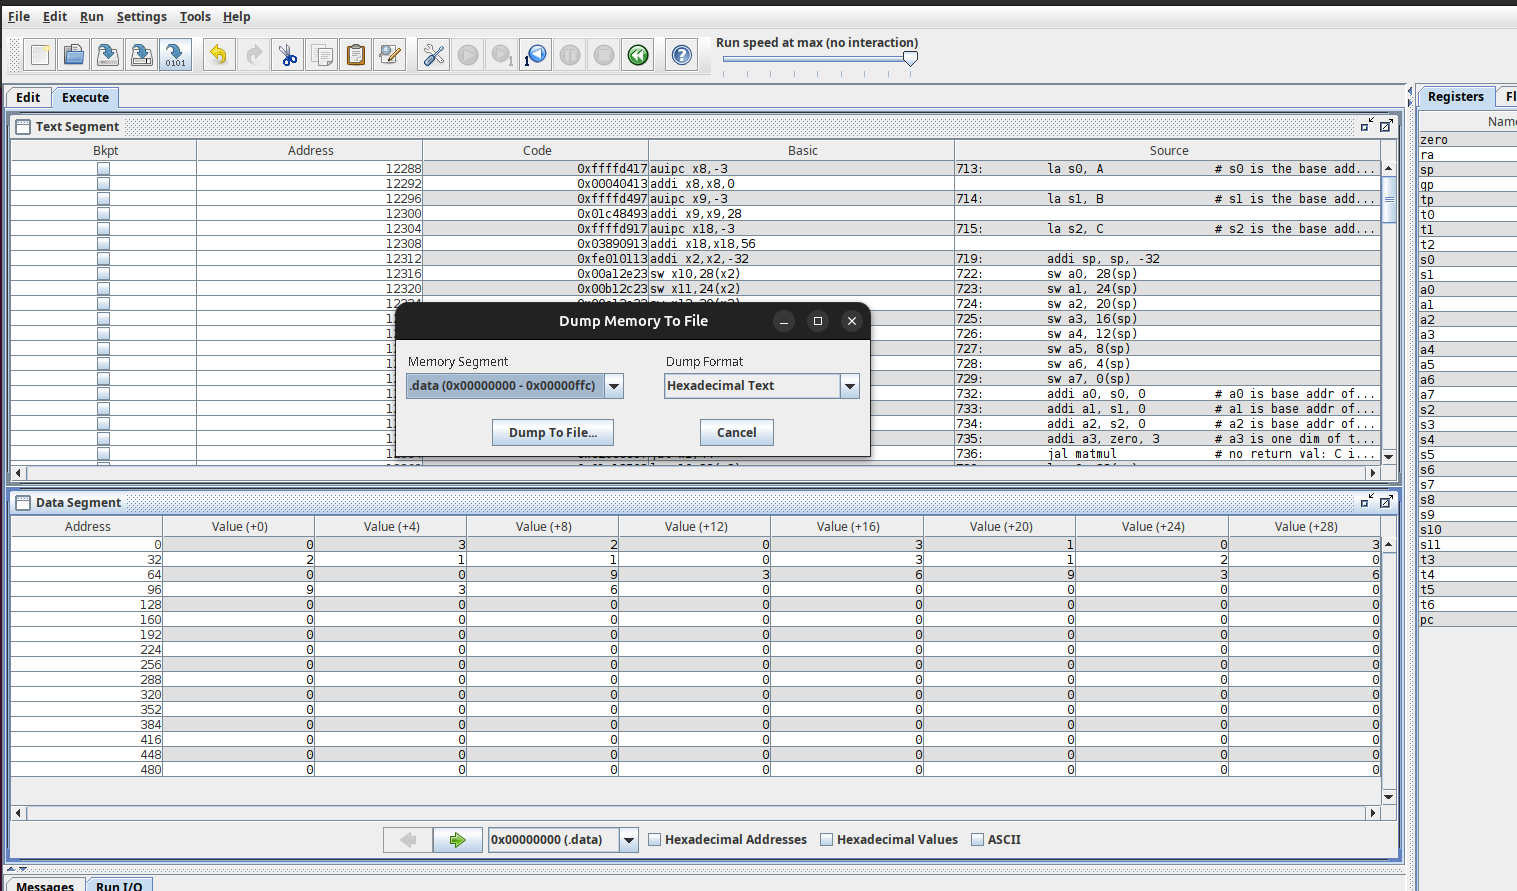
\includegraphics[width=0.8\textwidth]{./photos/RARS_config.png}
					\end{figure}

			\end{enumerate}	

		\section{Results}

			All \textsc{diff}s passed except for the $50 \times 50$ matrix. 
			The RISC-V OTTER memory mapping did not have enough memory to 
			store both matrices  $A, B$, throwing a compile time error.
			Below are the screenshots of the matrices in memory. It should
			be noted that const $M$ is set to a single dimension of the
			matrices. 

			\subsection{dataset3.h}
				\begin{figure}[H]
					\centering
					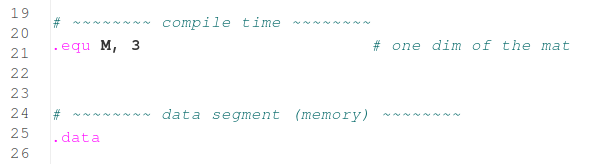
\includegraphics[width=0.5\textwidth]{./photos/m3.png}
				\end{figure}

				\begin{figure}[H]
					\centering
					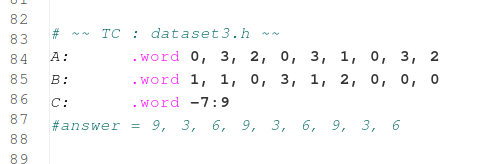
\includegraphics[width=0.6\textwidth]{./photos/input3.png}
				\end{figure}

				\begin{figure}[H]
					\centering
					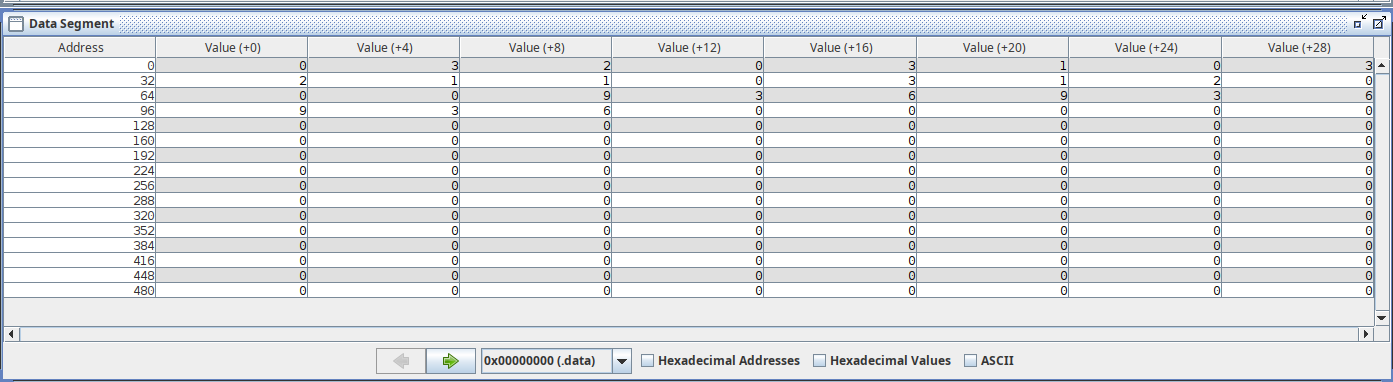
\includegraphics[width=0.9\textwidth]{./photos/result3.png}
				\end{figure}

			\subsection{dataset10.h}
				\begin{figure}[H]
					\centering
					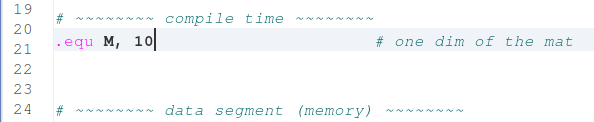
\includegraphics[width=0.5\textwidth]{./photos/m10.png}
				\end{figure}

				\begin{figure}[H]
					\centering
					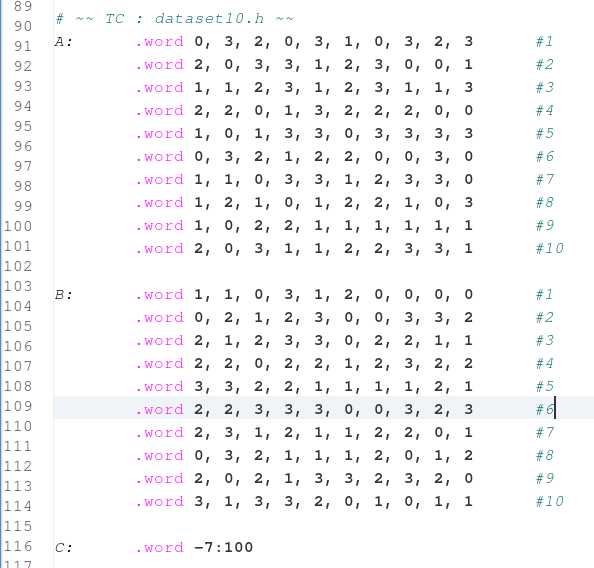
\includegraphics[width=0.6\textwidth]{./photos/input10.png}
				\end{figure}

				\begin{figure}[H]
					\centering
					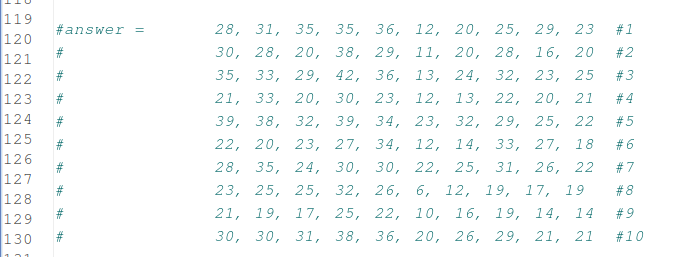
\includegraphics[width=0.6\textwidth]{./photos/input10a.png}
				\end{figure}

				\begin{figure}[H]
					\centering
					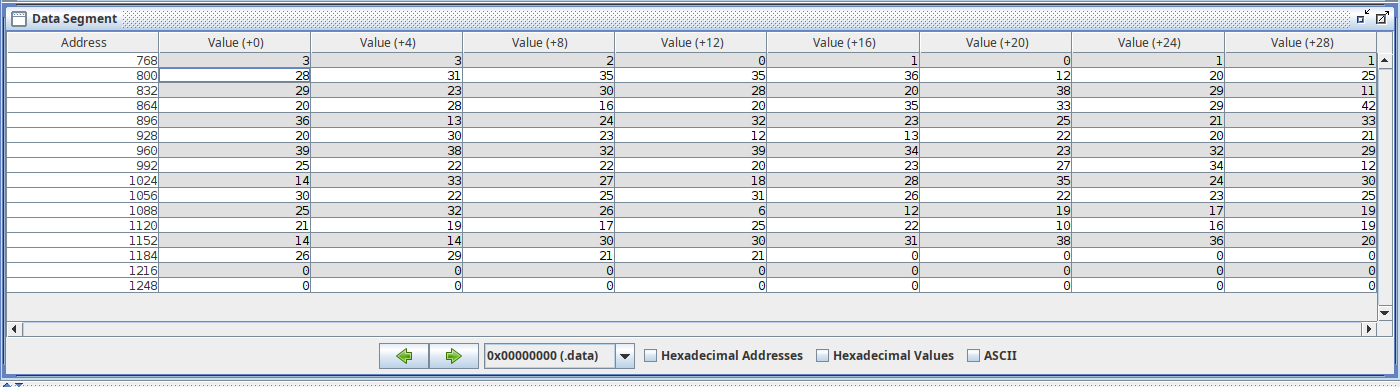
\includegraphics[width=0.9\textwidth]{./photos/result10.png}
				\end{figure}


			\subsection{dataset16.h}
				\begin{figure}[H]
					\centering
					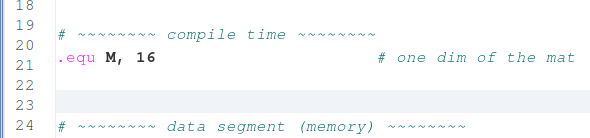
\includegraphics[width=0.5\textwidth]{./photos/m16.png}
				\end{figure}

				\begin{figure}[H]
					\centering
					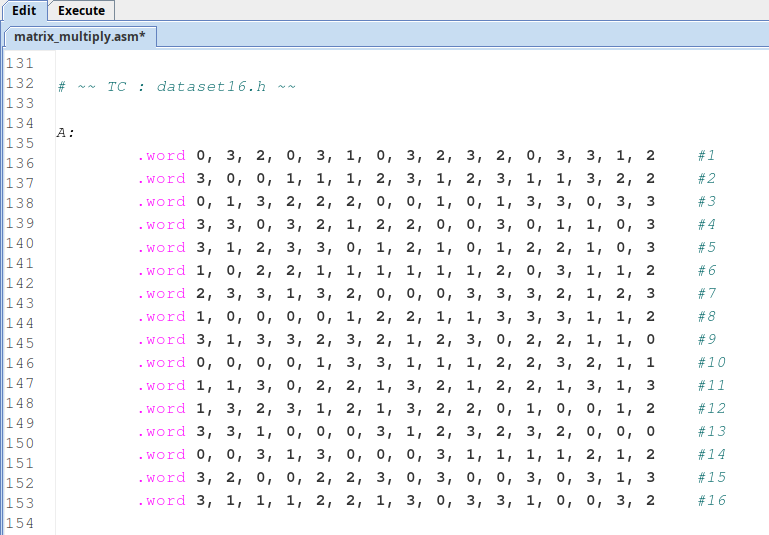
\includegraphics[width=0.6\textwidth]{./photos/input16a.png}
				\end{figure}

				\begin{figure}[H]
					\centering
					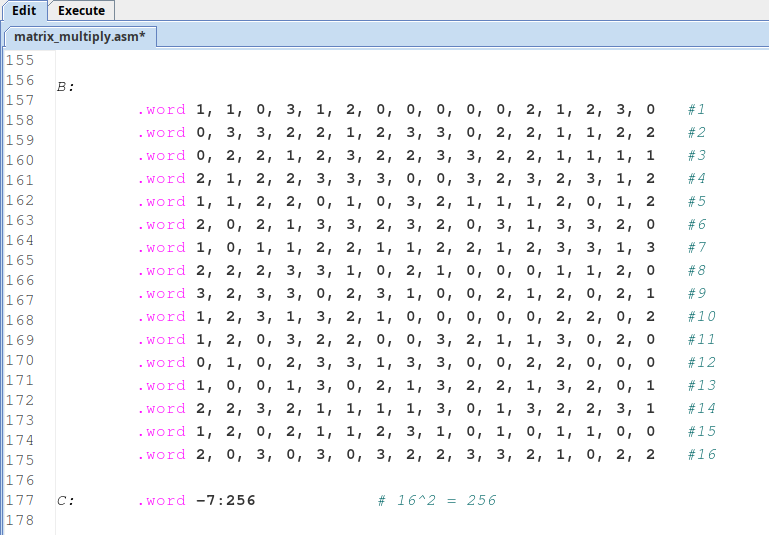
\includegraphics[width=0.6\textwidth]{./photos/input16b.png}
				\end{figure}

				\begin{figure}[H]
					\centering
					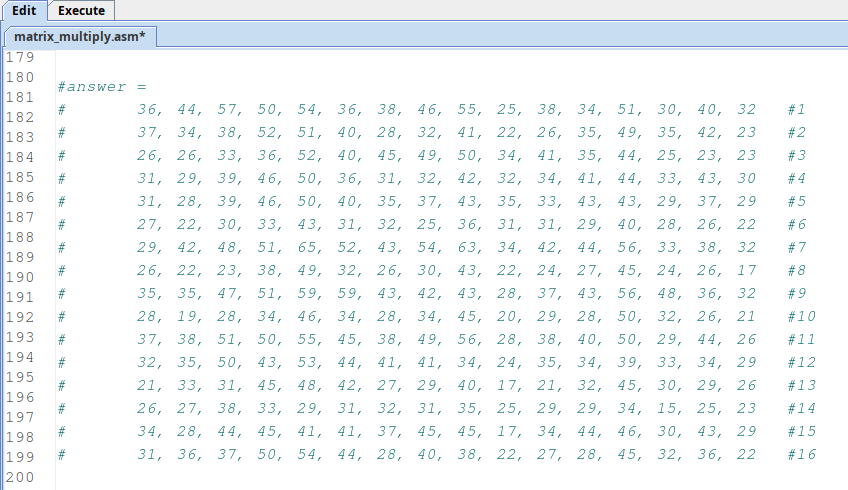
\includegraphics[width=0.6\textwidth]{./photos/input16c.png}
				\end{figure}

				\begin{figure}[H]
					\centering
					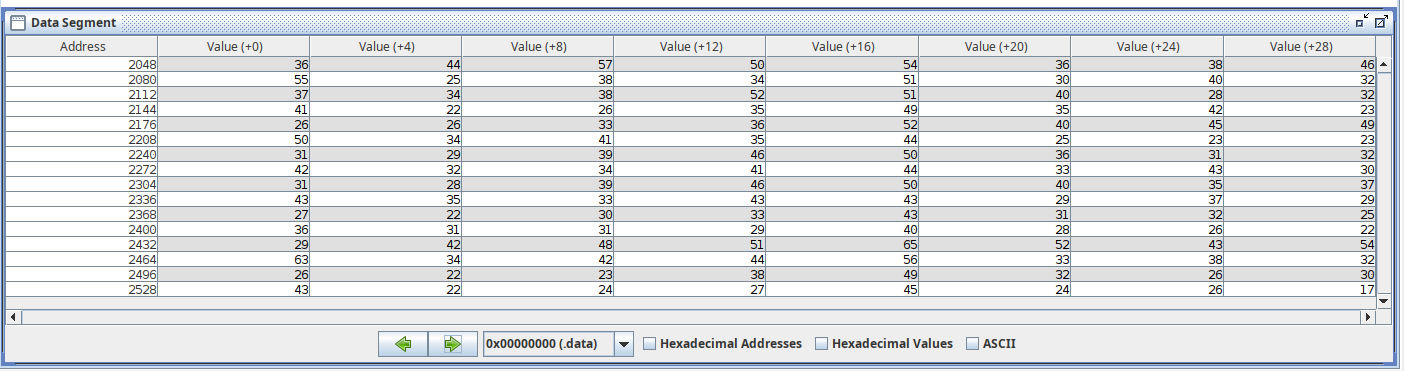
\includegraphics[width=0.9\textwidth]{./photos/result16a.png}
				\end{figure}

				\begin{figure}[H]
					\centering
					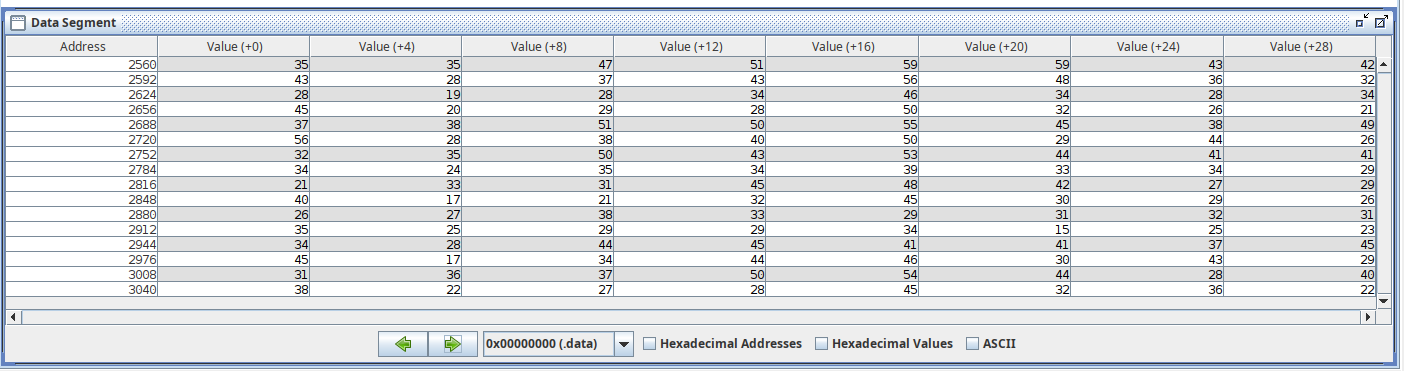
\includegraphics[width=0.9\textwidth]{./photos/result16b.png}
				\end{figure}

			\subsection{dataset50.h}
				Couldn't compile due to resource limitations. Skipped.  


			\subsection{Diff validation}
				\begin{figure}[H]
					\centering
					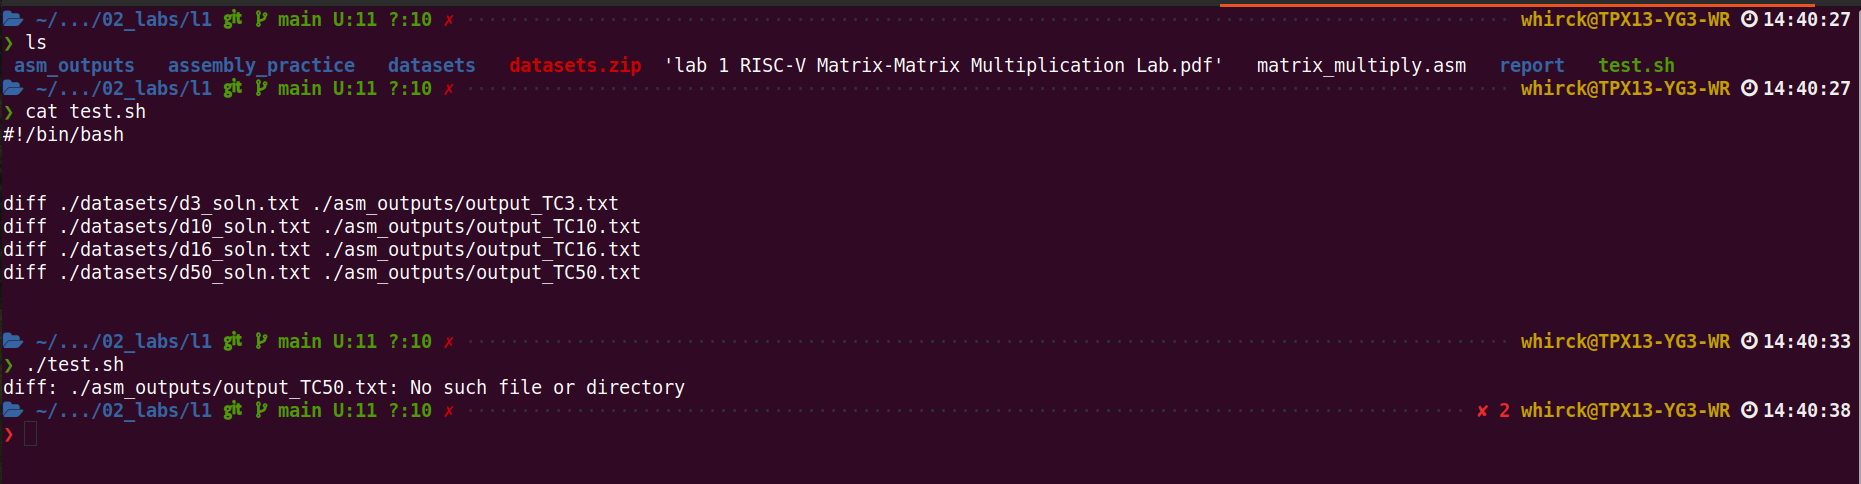
\includegraphics[width=0.8\textwidth]{./photos/shell.png}
					\caption{Shell validation using `diff`}
				\end{figure}


\end{document}
